\documentclass[1p]{elsarticle_modified}
%\bibliographystyle{elsarticle-num}

%\usepackage[colorlinks]{hyperref}
%\usepackage{abbrmath_seonhwa} %\Abb, \Ascr, \Acal ,\Abf, \Afrak
\usepackage{amsfonts}
\usepackage{amssymb}
\usepackage{amsmath}
\usepackage{amsthm}
\usepackage{scalefnt}
\usepackage{amsbsy}
\usepackage{kotex}
\usepackage{caption}
\usepackage{subfig}
\usepackage{color}
\usepackage{graphicx}
\usepackage{xcolor} %% white, black, red, green, blue, cyan, magenta, yellow
\usepackage{float}
\usepackage{setspace}
\usepackage{hyperref}

\usepackage{tikz}
\usetikzlibrary{arrows}

\usepackage{multirow}
\usepackage{array} % fixed length table
\usepackage{hhline}

%%%%%%%%%%%%%%%%%%%%%
\makeatletter
\renewcommand*\env@matrix[1][\arraystretch]{%
	\edef\arraystretch{#1}%
	\hskip -\arraycolsep
	\let\@ifnextchar\new@ifnextchar
	\array{*\c@MaxMatrixCols c}}
\makeatother %https://tex.stackexchange.com/questions/14071/how-can-i-increase-the-line-spacing-in-a-matrix
%%%%%%%%%%%%%%%

\usepackage[normalem]{ulem}

\newcommand{\msout}[1]{\ifmmode\text{\sout{\ensuremath{#1}}}\else\sout{#1}\fi}
%SOURCE: \msout is \stkout macro in https://tex.stackexchange.com/questions/20609/strikeout-in-math-mode

\newcommand{\cancel}[1]{
	\ifmmode
	{\color{red}\msout{#1}}
	\else
	{\color{red}\sout{#1}}
	\fi
}

\newcommand{\add}[1]{
	{\color{blue}\uwave{#1}}
}

\newcommand{\replace}[2]{
	\ifmmode
	{\color{red}\msout{#1}}{\color{blue}\uwave{#2}}
	\else
	{\color{red}\sout{#1}}{\color{blue}\uwave{#2}}
	\fi
}

\newcommand{\Sol}{\mathcal{S}} %segment
\newcommand{\D}{D} %diagram
\newcommand{\A}{\mathcal{A}} %arc


%%%%%%%%%%%%%%%%%%%%%%%%%%%%%5 test

\def\sl{\operatorname{\textup{SL}}(2,\Cbb)}
\def\psl{\operatorname{\textup{PSL}}(2,\Cbb)}
\def\quan{\mkern 1mu \triangleright \mkern 1mu}

\theoremstyle{definition}
\newtheorem{thm}{Theorem}[section]
\newtheorem{prop}[thm]{Proposition}
\newtheorem{lem}[thm]{Lemma}
\newtheorem{ques}[thm]{Question}
\newtheorem{cor}[thm]{Corollary}
\newtheorem{defn}[thm]{Definition}
\newtheorem{exam}[thm]{Example}
\newtheorem{rmk}[thm]{Remark}
\newtheorem{alg}[thm]{Algorithm}

\newcommand{\I}{\sqrt{-1}}
\begin{document}

%\begin{frontmatter}
%
%\title{Boundary parabolic representations of knots up to 8 crossings}
%
%%% Group authors per affiliation:
%\author{Yunhi Cho} 
%\address{Department of Mathematics, University of Seoul, Seoul, Korea}
%\ead{yhcho@uos.ac.kr}
%
%
%\author{Seonhwa Kim} %\fnref{s_kim}}
%\address{Center for Geometry and Physics, Institute for Basic Science, Pohang, 37673, Korea}
%\ead{ryeona17@ibs.re.kr}
%
%\author{Hyuk Kim}
%\address{Department of Mathematical Sciences, Seoul National University, Seoul 08826, Korea}
%\ead{hyukkim@snu.ac.kr}
%
%\author{Seokbeom Yoon}
%\address{Department of Mathematical Sciences, Seoul National University, Seoul, 08826,  Korea}
%\ead{sbyoon15@snu.ac.kr}
%
%\begin{abstract}
%We find all boundary parabolic representation of knots up to 8 crossings.
%
%\end{abstract}
%\begin{keyword}
%    \MSC[2010] 57M25 
%\end{keyword}
%
%\end{frontmatter}

%\linenumbers
%\tableofcontents
%
\newcommand\colored[1]{\textcolor{white}{\rule[-0.35ex]{0.8em}{1.4ex}}\kern-0.8em\color{red} #1}%
%\newcommand\colored[1]{\textcolor{white}{ #1}\kern-2.17ex	\textcolor{white}{ #1}\kern-1.81ex	\textcolor{white}{ #1}\kern-2.15ex\color{red}#1	}

{\Large $\underline{12a_{0221}~(K12a_{0221})}$}

\setlength{\tabcolsep}{10pt}
\renewcommand{\arraystretch}{1.6}
\vspace{1cm}\begin{tabular}{m{100pt}>{\centering\arraybackslash}m{274pt}}
\multirow{5}{120pt}{
	\centering
	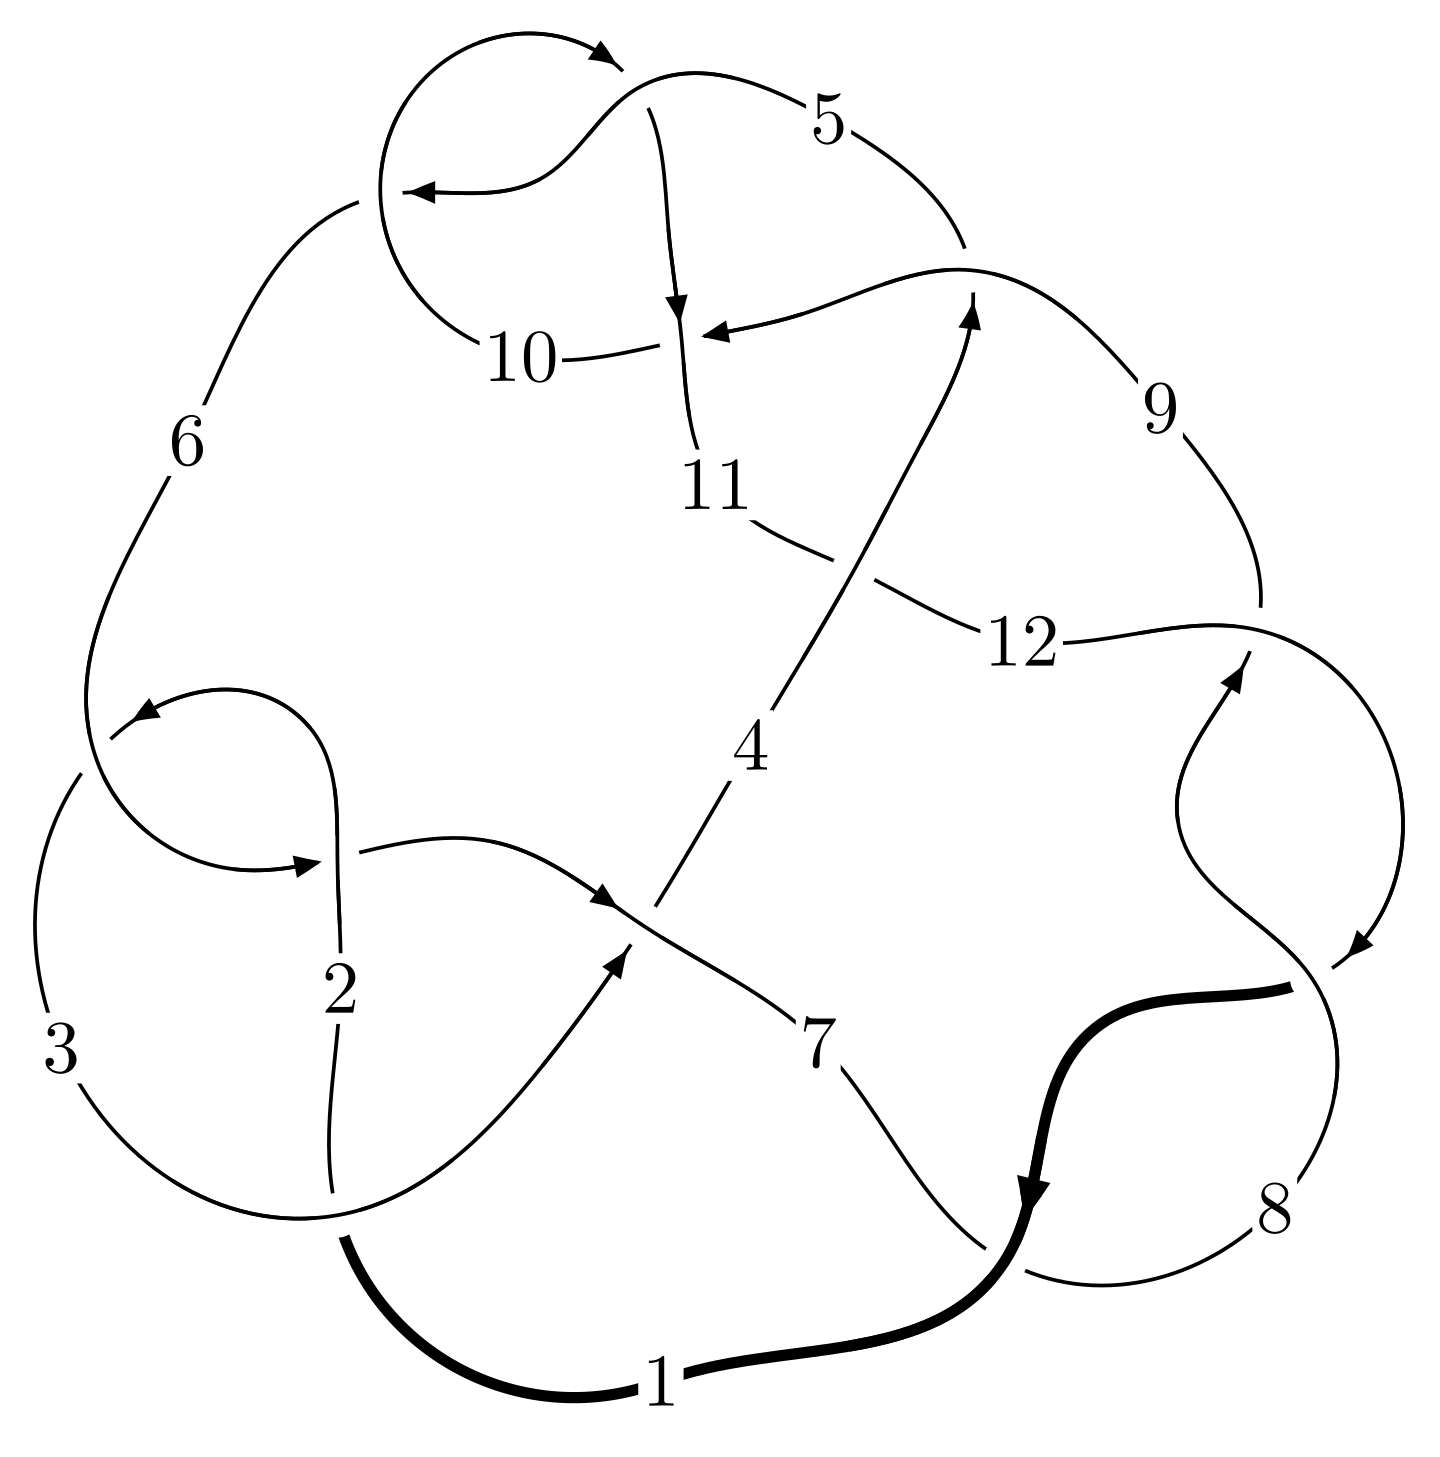
\includegraphics[width=112pt]{../../../GIT/diagram.site/Diagrams/png/1022_12a_0221.png}\\
\ \ \ A knot diagram\footnotemark}&
\allowdisplaybreaks
\textbf{Linearized knot diagam} \\
\cline{2-2}
 &
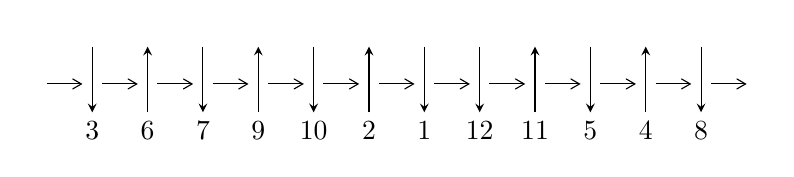
\begin{tikzpicture}[x=20pt, y=17pt]
	% nodes
	\node (C0) at (0, 0) {};
	\node (C1) at (1, 0) {};
	\node (C1U) at (1, +1) {};
	\node (C1D) at (1, -1) {3};

	\node (C2) at (2, 0) {};
	\node (C2U) at (2, +1) {};
	\node (C2D) at (2, -1) {6};

	\node (C3) at (3, 0) {};
	\node (C3U) at (3, +1) {};
	\node (C3D) at (3, -1) {7};

	\node (C4) at (4, 0) {};
	\node (C4U) at (4, +1) {};
	\node (C4D) at (4, -1) {9};

	\node (C5) at (5, 0) {};
	\node (C5U) at (5, +1) {};
	\node (C5D) at (5, -1) {10};

	\node (C6) at (6, 0) {};
	\node (C6U) at (6, +1) {};
	\node (C6D) at (6, -1) {2};

	\node (C7) at (7, 0) {};
	\node (C7U) at (7, +1) {};
	\node (C7D) at (7, -1) {1};

	\node (C8) at (8, 0) {};
	\node (C8U) at (8, +1) {};
	\node (C8D) at (8, -1) {12};

	\node (C9) at (9, 0) {};
	\node (C9U) at (9, +1) {};
	\node (C9D) at (9, -1) {11};

	\node (C10) at (10, 0) {};
	\node (C10U) at (10, +1) {};
	\node (C10D) at (10, -1) {5};

	\node (C11) at (11, 0) {};
	\node (C11U) at (11, +1) {};
	\node (C11D) at (11, -1) {4};

	\node (C12) at (12, 0) {};
	\node (C12U) at (12, +1) {};
	\node (C12D) at (12, -1) {8};
	\node (C13) at (13, 0) {};

	% arrows
	\draw[->,>={angle 60}]
	(C0) edge (C1) (C1) edge (C2) (C2) edge (C3) (C3) edge (C4) (C4) edge (C5) (C5) edge (C6) (C6) edge (C7) (C7) edge (C8) (C8) edge (C9) (C9) edge (C10) (C10) edge (C11) (C11) edge (C12) (C12) edge (C13) ;	\draw[->,>=stealth]
	(C1U) edge (C1D) (C2D) edge (C2U) (C3U) edge (C3D) (C4D) edge (C4U) (C5U) edge (C5D) (C6D) edge (C6U) (C7U) edge (C7D) (C8U) edge (C8D) (C9D) edge (C9U) (C10U) edge (C10D) (C11D) edge (C11U) (C12U) edge (C12D) ;
	\end{tikzpicture} \\
\hhline{~~} \\& 
\textbf{Solving Sequence} \\ \cline{2-2} 
 &
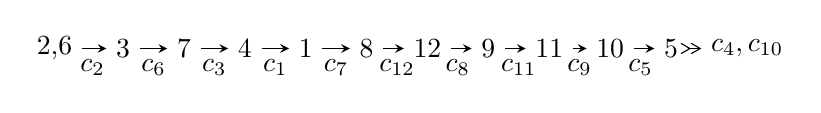
\begin{tikzpicture}[x=22pt, y=7pt]
	% node
	\node (A0) at (-1/8, 0) {2,6};
	\node (A1) at (1, 0) {3};
	\node (A2) at (2, 0) {7};
	\node (A3) at (3, 0) {4};
	\node (A4) at (4, 0) {1};
	\node (A5) at (5, 0) {8};
	\node (A6) at (6, 0) {12};
	\node (A7) at (7, 0) {9};
	\node (A8) at (8, 0) {11};
	\node (A9) at (9, 0) {10};
	\node (A10) at (10, 0) {5};
	\node (C1) at (1/2, -1) {$c_{2}$};
	\node (C2) at (3/2, -1) {$c_{6}$};
	\node (C3) at (5/2, -1) {$c_{3}$};
	\node (C4) at (7/2, -1) {$c_{1}$};
	\node (C5) at (9/2, -1) {$c_{7}$};
	\node (C6) at (11/2, -1) {$c_{12}$};
	\node (C7) at (13/2, -1) {$c_{8}$};
	\node (C8) at (15/2, -1) {$c_{11}$};
	\node (C9) at (17/2, -1) {$c_{9}$};
	\node (C10) at (19/2, -1) {$c_{5}$};
	\node (A11) at (45/4, 0) {$c_{4},c_{10}$};

	% edge
	\draw[->,>=stealth]	
	(A0) edge (A1) (A1) edge (A2) (A2) edge (A3) (A3) edge (A4) (A4) edge (A5) (A5) edge (A6) (A6) edge (A7) (A7) edge (A8) (A8) edge (A9) (A9) edge (A10) ;
	\draw[->>,>={angle 60}]	
	(A10) edge (A11);
\end{tikzpicture} \\ 

\end{tabular} \\

\footnotetext{
The image of knot diagram is generated by the software ``\textbf{Draw programme}" developed by Andrew Bartholomew(\url{http://www.layer8.co.uk/maths/draw/index.htm\#Running-draw}), where we modified some parts for our purpose(\url{https://github.com/CATsTAILs/LinksPainter}).
}\phantom \\ \newline 
\centering \textbf{Ideals for irreducible components\footnotemark of $X_{\text{par}}$} 
 
\begin{align*}
I^u_{1}&=\langle 
u^{84}+u^{83}+\cdots+2 u+1\rangle \\
\\
\end{align*}
\raggedright * 1 irreducible components of $\dim_{\mathbb{C}}=0$, with total 84 representations.\\
\footnotetext{All coefficients of polynomials are rational numbers. But the coefficients are sometimes approximated in decimal forms when there is not enough margin.}
\newpage
\renewcommand{\arraystretch}{1}
\centering \section*{I. $I^u_{1}= \langle u^{84}+u^{83}+\cdots+2 u+1 \rangle$}
\flushleft \textbf{(i) Arc colorings}\\
\begin{tabular}{m{7pt} m{180pt} m{7pt} m{180pt} }
\flushright $a_{2}=$&$\begin{pmatrix}1\\0\end{pmatrix}$ \\
\flushright $a_{6}=$&$\begin{pmatrix}0\\u\end{pmatrix}$ \\
\flushright $a_{3}=$&$\begin{pmatrix}1\\- u^2\end{pmatrix}$ \\
\flushright $a_{7}=$&$\begin{pmatrix}u\\u\end{pmatrix}$ \\
\flushright $a_{4}=$&$\begin{pmatrix}u^4+u^2+1\\u^4\end{pmatrix}$ \\
\flushright $a_{1}=$&$\begin{pmatrix}u^2+1\\- u^4\end{pmatrix}$ \\
\flushright $a_{8}=$&$\begin{pmatrix}- u^7-2 u^5-2 u^3\\u^9+u^7+u^5+u\end{pmatrix}$ \\
\flushright $a_{12}=$&$\begin{pmatrix}u^{12}+3 u^{10}+5 u^8+4 u^6+2 u^4+u^2+1\\- u^{14}-2 u^{12}-3 u^{10}-2 u^8-2 u^6-2 u^4- u^2\end{pmatrix}$ \\
\flushright $a_{9}=$&$\begin{pmatrix}- u^{17}-4 u^{15}-9 u^{13}-12 u^{11}-11 u^9-8 u^7-6 u^5-4 u^3- u\\u^{19}+3 u^{17}+6 u^{15}+7 u^{13}+7 u^{11}+7 u^9+6 u^7+4 u^5+u^3+u\end{pmatrix}$ \\
\flushright $a_{11}=$&$\begin{pmatrix}u^{22}+5 u^{20}+\cdots+2 u^2+1\\u^{22}+4 u^{20}+9 u^{18}+12 u^{16}+10 u^{14}+6 u^{12}+3 u^{10}+2 u^8- u^6-2 u^4- u^2\end{pmatrix}$ \\
\flushright $a_{10}=$&$\begin{pmatrix}u^{63}+14 u^{61}+\cdots+56 u^7+12 u^5\\u^{63}+13 u^{61}+\cdots-6 u^7+u\end{pmatrix}$ \\
\flushright $a_{5}=$&$\begin{pmatrix}u^{40}+9 u^{38}+\cdots+2 u^2+1\\- u^{42}-8 u^{40}+\cdots-2 u^4- u^2\end{pmatrix}$\\&\end{tabular}
\flushleft \textbf{(ii) Obstruction class $= -1$}\\~\\
\flushleft \textbf{(iii) Cusp Shapes $= 4 u^{83}+4 u^{82}+\cdots+12 u+6$}\\~\\
\newpage\renewcommand{\arraystretch}{1}
\flushleft \textbf{(iv) u-Polynomials at the component}\newline \\
\begin{tabular}{m{50pt}|m{274pt}}
Crossings & \hspace{64pt}u-Polynomials at each crossing \\
\hline $$\begin{aligned}c_{1}\end{aligned}$$&$\begin{aligned}
&u^{84}+37 u^{83}+\cdots+2 u+1
\end{aligned}$\\
\hline $$\begin{aligned}c_{2},c_{6}\end{aligned}$$&$\begin{aligned}
&u^{84}- u^{83}+\cdots-2 u+1
\end{aligned}$\\
\hline $$\begin{aligned}c_{3}\end{aligned}$$&$\begin{aligned}
&u^{84}+u^{83}+\cdots-2 u+1
\end{aligned}$\\
\hline $$\begin{aligned}c_{4}\end{aligned}$$&$\begin{aligned}
&u^{84}+u^{83}+\cdots-1110 u+1237
\end{aligned}$\\
\hline $$\begin{aligned}c_{5},c_{10}\end{aligned}$$&$\begin{aligned}
&u^{84}- u^{83}+\cdots+u^2+1
\end{aligned}$\\
\hline $$\begin{aligned}c_{7},c_{8},c_{12}\end{aligned}$$&$\begin{aligned}
&u^{84}-5 u^{83}+\cdots-150 u+13
\end{aligned}$\\
\hline $$\begin{aligned}c_{9}\end{aligned}$$&$\begin{aligned}
&u^{84}-41 u^{83}+\cdots-2 u+1
\end{aligned}$\\
\hline $$\begin{aligned}c_{11}\end{aligned}$$&$\begin{aligned}
&u^{84}-5 u^{83}+\cdots-20 u+133
\end{aligned}$\\
\hline
\end{tabular}\\~\\
\newpage\renewcommand{\arraystretch}{1}
\flushleft \textbf{(v) Riley Polynomials at the component}\newline \\
\begin{tabular}{m{50pt}|m{274pt}}
Crossings & \hspace{64pt}Riley Polynomials at each crossing \\
\hline $$\begin{aligned}c_{1}\end{aligned}$$&$\begin{aligned}
&y^{84}+21 y^{83}+\cdots+10 y+1
\end{aligned}$\\
\hline $$\begin{aligned}c_{2},c_{6}\end{aligned}$$&$\begin{aligned}
&y^{84}+37 y^{83}+\cdots+2 y+1
\end{aligned}$\\
\hline $$\begin{aligned}c_{3}\end{aligned}$$&$\begin{aligned}
&y^{84}+5 y^{83}+\cdots+66 y+1
\end{aligned}$\\
\hline $$\begin{aligned}c_{4}\end{aligned}$$&$\begin{aligned}
&y^{84}-31 y^{83}+\cdots-27364962 y+1530169
\end{aligned}$\\
\hline $$\begin{aligned}c_{5},c_{10}\end{aligned}$$&$\begin{aligned}
&y^{84}+41 y^{83}+\cdots+2 y+1
\end{aligned}$\\
\hline $$\begin{aligned}c_{7},c_{8},c_{12}\end{aligned}$$&$\begin{aligned}
&y^{84}+89 y^{83}+\cdots+11742 y+169
\end{aligned}$\\
\hline $$\begin{aligned}c_{9}\end{aligned}$$&$\begin{aligned}
&y^{84}+5 y^{83}+\cdots+10 y+1
\end{aligned}$\\
\hline $$\begin{aligned}c_{11}\end{aligned}$$&$\begin{aligned}
&y^{84}-11 y^{83}+\cdots+78070 y+17689
\end{aligned}$\\
\hline
\end{tabular}\\~\\
\newpage\flushleft \textbf{(vi) Complex Volumes and Cusp Shapes}
$$\begin{array}{c|c|c}  
\text{Solutions to }I^u_{1}& \I (\text{vol} + \sqrt{-1}CS) & \text{Cusp shape}\\
 \hline 
\begin{aligned}
u &= -0.223462 + 0.933764 I\end{aligned}
 & -0.07570 - 1.69164 I & \phantom{-0.000000 } 0 \\ \hline\begin{aligned}
u &= -0.223462 - 0.933764 I\end{aligned}
 & -0.07570 + 1.69164 I & \phantom{-0.000000 } 0 \\ \hline\begin{aligned}
u &= \phantom{-}0.791209 + 0.516161 I\end{aligned}
 & \phantom{-}10.32730 + 7.27403 I & \phantom{-}5.32581 - 5.73192 I \\ \hline\begin{aligned}
u &= \phantom{-}0.791209 - 0.516161 I\end{aligned}
 & \phantom{-}10.32730 - 7.27403 I & \phantom{-}5.32581 + 5.73192 I \\ \hline\begin{aligned}
u &= \phantom{-}0.037106 + 1.056750 I\end{aligned}
 & -0.19944 - 2.21631 I & \phantom{-0.000000 } 0 \\ \hline\begin{aligned}
u &= \phantom{-}0.037106 - 1.056750 I\end{aligned}
 & -0.19944 + 2.21631 I & \phantom{-0.000000 } 0 \\ \hline\begin{aligned}
u &= \phantom{-}0.796662 + 0.503525 I\end{aligned}
 & \phantom{-}12.03280 - 0.97322 I & \phantom{-}7.54914 + 0. I\phantom{ +0.000000I} \\ \hline\begin{aligned}
u &= \phantom{-}0.796662 - 0.503525 I\end{aligned}
 & \phantom{-}12.03280 + 0.97322 I & \phantom{-}7.54914 + 0. I\phantom{ +0.000000I} \\ \hline\begin{aligned}
u &= -0.787400 + 0.509956 I\end{aligned}
 & \phantom{-}7.67805 - 2.34302 I & \phantom{-0.000000 } 0 \\ \hline\begin{aligned}
u &= -0.787400 - 0.509956 I\end{aligned}
 & \phantom{-}7.67805 + 2.34302 I & \phantom{-0.000000 } 0 \\ \hline\begin{aligned}
u &= \phantom{-}0.543765 + 0.916385 I\end{aligned}
 & \phantom{-}2.63357 - 1.71163 I & \phantom{-0.000000 } 0 \\ \hline\begin{aligned}
u &= \phantom{-}0.543765 - 0.916385 I\end{aligned}
 & \phantom{-}2.63357 + 1.71163 I & \phantom{-0.000000 } 0 \\ \hline\begin{aligned}
u &= -0.805009 + 0.474254 I\end{aligned}
 & \phantom{-}11.86550 + 2.32230 I & \phantom{-}7.32986 + 0. I\phantom{ +0.000000I} \\ \hline\begin{aligned}
u &= -0.805009 - 0.474254 I\end{aligned}
 & \phantom{-}11.86550 - 2.32230 I & \phantom{-}7.32986 + 0. I\phantom{ +0.000000I} \\ \hline\begin{aligned}
u &= -0.807000 + 0.462064 I\end{aligned}
 & \phantom{-}10.0185 + 10.5475 I & \phantom{-}4.83061 - 6.04400 I \\ \hline\begin{aligned}
u &= -0.807000 - 0.462064 I\end{aligned}
 & \phantom{-}10.0185 - 10.5475 I & \phantom{-}4.83061 + 6.04400 I \\ \hline\begin{aligned}
u &= -0.508321 + 0.945367 I\end{aligned}
 & \phantom{-}0.05765 - 2.39517 I & \phantom{-0.000000 } 0 \\ \hline\begin{aligned}
u &= -0.508321 - 0.945367 I\end{aligned}
 & \phantom{-}0.05765 + 2.39517 I & \phantom{-0.000000 } 0 \\ \hline\begin{aligned}
u &= \phantom{-}0.801408 + 0.464683 I\end{aligned}
 & \phantom{-}7.42012 - 5.56366 I & \phantom{-0.000000 -}0. + 2.51060 I \\ \hline\begin{aligned}
u &= \phantom{-}0.801408 - 0.464683 I\end{aligned}
 & \phantom{-}7.42012 + 5.56366 I & \phantom{-0.000000 } 0. - 2.51060 I \\ \hline\begin{aligned}
u &= \phantom{-}0.308336 + 1.036850 I\end{aligned}
 & -3.73977 - 0.08549 I & \phantom{-0.000000 } 0 \\ \hline\begin{aligned}
u &= \phantom{-}0.308336 - 1.036850 I\end{aligned}
 & -3.73977 + 0.08549 I & \phantom{-0.000000 } 0 \\ \hline\begin{aligned}
u &= -0.285037 + 1.047880 I\end{aligned}
 & -1.75442 + 4.74800 I & \phantom{-0.000000 } 0 \\ \hline\begin{aligned}
u &= -0.285037 - 1.047880 I\end{aligned}
 & -1.75442 - 4.74800 I & \phantom{-0.000000 } 0 \\ \hline\begin{aligned}
u &= -0.769820 + 0.487123 I\end{aligned}
 & \phantom{-}5.19035 - 0.86260 I & \phantom{-}1.23878 + 3.04762 I \\ \hline\begin{aligned}
u &= -0.769820 - 0.487123 I\end{aligned}
 & \phantom{-}5.19035 + 0.86260 I & \phantom{-}1.23878 - 3.04762 I \\ \hline\begin{aligned}
u &= \phantom{-}0.778145 + 0.470305 I\end{aligned}
 & \phantom{-}5.09099 - 3.85034 I & \phantom{-}0.89323 + 3.65261 I \\ \hline\begin{aligned}
u &= \phantom{-}0.778145 - 0.470305 I\end{aligned}
 & \phantom{-}5.09099 + 3.85034 I & \phantom{-}0.89323 - 3.65261 I \\ \hline\begin{aligned}
u &= -0.339809 + 0.830779 I\end{aligned}
 & -0.13330 - 1.63331 I & -0.57375 + 3.86192 I \\ \hline\begin{aligned}
u &= -0.339809 - 0.830779 I\end{aligned}
 & -0.13330 + 1.63331 I & -0.57375 - 3.86192 I\\
 \hline 
 \end{array}$$\newpage$$\begin{array}{c|c|c}  
\text{Solutions to }I^u_{1}& \I (\text{vol} + \sqrt{-1}CS) & \text{Cusp shape}\\
 \hline 
\begin{aligned}
u &= \phantom{-}0.358186 + 1.043080 I\end{aligned}
 & -4.14324 + 1.55939 I & \phantom{-0.000000 } 0 \\ \hline\begin{aligned}
u &= \phantom{-}0.358186 - 1.043080 I\end{aligned}
 & -4.14324 - 1.55939 I & \phantom{-0.000000 } 0 \\ \hline\begin{aligned}
u &= \phantom{-}0.043589 + 1.113230 I\end{aligned}
 & \phantom{-}1.93267 - 3.70749 I & \phantom{-0.000000 } 0 \\ \hline\begin{aligned}
u &= \phantom{-}0.043589 - 1.113230 I\end{aligned}
 & \phantom{-}1.93267 + 3.70749 I & \phantom{-0.000000 } 0 \\ \hline\begin{aligned}
u &= \phantom{-}0.551965 + 0.969258 I\end{aligned}
 & \phantom{-}3.24663 + 5.73101 I & \phantom{-0.000000 } 0 \\ \hline\begin{aligned}
u &= \phantom{-}0.551965 - 0.969258 I\end{aligned}
 & \phantom{-}3.24663 - 5.73101 I & \phantom{-0.000000 } 0 \\ \hline\begin{aligned}
u &= -0.026149 + 1.121100 I\end{aligned}
 & \phantom{-}6.27570 + 0.52297 I & \phantom{-0.000000 } 0 \\ \hline\begin{aligned}
u &= -0.026149 - 1.121100 I\end{aligned}
 & \phantom{-}6.27570 - 0.52297 I & \phantom{-0.000000 } 0 \\ \hline\begin{aligned}
u &= -0.381786 + 1.056500 I\end{aligned}
 & -2.57890 - 6.08174 I & \phantom{-0.000000 } 0 \\ \hline\begin{aligned}
u &= -0.381786 - 1.056500 I\end{aligned}
 & -2.57890 + 6.08174 I & \phantom{-0.000000 } 0 \\ \hline\begin{aligned}
u &= -0.047926 + 1.123680 I\end{aligned}
 & \phantom{-}4.49933 + 8.62941 I & \phantom{-0.000000 } 0 \\ \hline\begin{aligned}
u &= -0.047926 - 1.123680 I\end{aligned}
 & \phantom{-}4.49933 - 8.62941 I & \phantom{-0.000000 } 0 \\ \hline\begin{aligned}
u &= \phantom{-}0.564858 + 0.667954 I\end{aligned}
 & \phantom{-}3.34666 + 6.18409 I & \phantom{-}4.75304 - 7.47482 I \\ \hline\begin{aligned}
u &= \phantom{-}0.564858 - 0.667954 I\end{aligned}
 & \phantom{-}3.34666 - 6.18409 I & \phantom{-}4.75304 + 7.47482 I \\ \hline\begin{aligned}
u &= -0.458432 + 1.061660 I\end{aligned}
 & -2.07874 - 0.79068 I & \phantom{-0.000000 } 0 \\ \hline\begin{aligned}
u &= -0.458432 - 1.061660 I\end{aligned}
 & -2.07874 + 0.79068 I & \phantom{-0.000000 } 0 \\ \hline\begin{aligned}
u &= \phantom{-}0.483376 + 1.064070 I\end{aligned}
 & -3.30588 + 5.23729 I & \phantom{-0.000000 } 0 \\ \hline\begin{aligned}
u &= \phantom{-}0.483376 - 1.064070 I\end{aligned}
 & -3.30588 - 5.23729 I & \phantom{-0.000000 } 0 \\ \hline\begin{aligned}
u &= -0.510868 + 0.650088 I\end{aligned}
 & \phantom{-}0.91179 - 1.80281 I & \phantom{-}1.30059 + 3.91326 I \\ \hline\begin{aligned}
u &= -0.510868 - 0.650088 I\end{aligned}
 & \phantom{-}0.91179 + 1.80281 I & \phantom{-}1.30059 - 3.91326 I \\ \hline\begin{aligned}
u &= -0.534113 + 1.054150 I\end{aligned}
 & \phantom{-}1.75841 - 4.59094 I & \phantom{-0.000000 } 0 \\ \hline\begin{aligned}
u &= -0.534113 - 1.054150 I\end{aligned}
 & \phantom{-}1.75841 + 4.59094 I & \phantom{-0.000000 } 0 \\ \hline\begin{aligned}
u &= \phantom{-}0.575651 + 0.581028 I\end{aligned}
 & \phantom{-}4.35803 - 1.20708 I & \phantom{-}6.98007 + 0.38131 I \\ \hline\begin{aligned}
u &= \phantom{-}0.575651 - 0.581028 I\end{aligned}
 & \phantom{-}4.35803 + 1.20708 I & \phantom{-}6.98007 - 0.38131 I \\ \hline\begin{aligned}
u &= \phantom{-}0.513175 + 1.074520 I\end{aligned}
 & -2.37945 + 6.93925 I & \phantom{-0.000000 } 0 \\ \hline\begin{aligned}
u &= \phantom{-}0.513175 - 1.074520 I\end{aligned}
 & -2.37945 - 6.93925 I & \phantom{-0.000000 } 0 \\ \hline\begin{aligned}
u &= -0.521503 + 1.082880 I\end{aligned}
 & -0.20890 - 11.73350 I & \phantom{-0.000000 } 0 \\ \hline\begin{aligned}
u &= -0.521503 - 1.082880 I\end{aligned}
 & -0.20890 + 11.73350 I & \phantom{-0.000000 } 0 \\ \hline\begin{aligned}
u &= -0.616198 + 1.072140 I\end{aligned}
 & \phantom{-}3.44700 - 4.37796 I & \phantom{-0.000000 } 0 \\ \hline\begin{aligned}
u &= -0.616198 - 1.072140 I\end{aligned}
 & \phantom{-}3.44700 + 4.37796 I & \phantom{-0.000000 } 0\\
 \hline 
 \end{array}$$\newpage$$\begin{array}{c|c|c}  
\text{Solutions to }I^u_{1}& \I (\text{vol} + \sqrt{-1}CS) & \text{Cusp shape}\\
 \hline 
\begin{aligned}
u &= -0.632761 + 1.065390 I\end{aligned}
 & \phantom{-}6.01874 - 3.00258 I & \phantom{-0.000000 } 0 \\ \hline\begin{aligned}
u &= -0.632761 - 1.065390 I\end{aligned}
 & \phantom{-}6.01874 + 3.00258 I & \phantom{-0.000000 } 0 \\ \hline\begin{aligned}
u &= \phantom{-}0.637028 + 1.063380 I\end{aligned}
 & \phantom{-}8.69167 - 1.90319 I & \phantom{-0.000000 } 0 \\ \hline\begin{aligned}
u &= \phantom{-}0.637028 - 1.063380 I\end{aligned}
 & \phantom{-}8.69167 + 1.90319 I & \phantom{-0.000000 } 0 \\ \hline\begin{aligned}
u &= \phantom{-}0.616009 + 1.082200 I\end{aligned}
 & \phantom{-}3.26859 + 9.11086 I & \phantom{-0.000000 } 0 \\ \hline\begin{aligned}
u &= \phantom{-}0.616009 - 1.082200 I\end{aligned}
 & \phantom{-}3.26859 - 9.11086 I & \phantom{-0.000000 } 0 \\ \hline\begin{aligned}
u &= \phantom{-}0.635377 + 1.071920 I\end{aligned}
 & \phantom{-}10.33310 + 6.35256 I & \phantom{-0.000000 } 0 \\ \hline\begin{aligned}
u &= \phantom{-}0.635377 - 1.071920 I\end{aligned}
 & \phantom{-}10.33310 - 6.35256 I & \phantom{-0.000000 } 0 \\ \hline\begin{aligned}
u &= -0.628985 + 1.088730 I\end{aligned}
 & \phantom{-}10.02760 - 7.69935 I & \phantom{-0.000000 } 0 \\ \hline\begin{aligned}
u &= -0.628985 - 1.088730 I\end{aligned}
 & \phantom{-}10.02760 + 7.69935 I & \phantom{-0.000000 } 0 \\ \hline\begin{aligned}
u &= \phantom{-}0.624160 + 1.091740 I\end{aligned}
 & \phantom{-}5.54652 + 10.91310 I & \phantom{-0.000000 } 0 \\ \hline\begin{aligned}
u &= \phantom{-}0.624160 - 1.091740 I\end{aligned}
 & \phantom{-}5.54652 - 10.91310 I & \phantom{-0.000000 } 0 \\ \hline\begin{aligned}
u &= -0.625644 + 1.094730 I\end{aligned}
 & \phantom{-}8.1266 - 15.9167 I & \phantom{-0.000000 } 0 \\ \hline\begin{aligned}
u &= -0.625644 - 1.094730 I\end{aligned}
 & \phantom{-}8.1266 + 15.9167 I & \phantom{-0.000000 } 0 \\ \hline\begin{aligned}
u &= -0.607812 + 0.381445 I\end{aligned}
 & \phantom{-}3.64708 + 0.08854 I & \phantom{-}5.69951 - 0.71462 I \\ \hline\begin{aligned}
u &= -0.607812 - 0.381445 I\end{aligned}
 & \phantom{-}3.64708 - 0.08854 I & \phantom{-}5.69951 + 0.71462 I \\ \hline\begin{aligned}
u &= -0.632909 + 0.297597 I\end{aligned}
 & \phantom{-}1.98999 + 7.25331 I & \phantom{-}1.90672 - 7.55824 I \\ \hline\begin{aligned}
u &= -0.632909 - 0.297597 I\end{aligned}
 & \phantom{-}1.98999 - 7.25331 I & \phantom{-}1.90672 + 7.55824 I \\ \hline\begin{aligned}
u &= \phantom{-}0.594633 + 0.293043 I\end{aligned}
 & -0.22402 - 2.57780 I & -1.72559 + 3.89319 I \\ \hline\begin{aligned}
u &= \phantom{-}0.594633 - 0.293043 I\end{aligned}
 & -0.22402 + 2.57780 I & -1.72559 - 3.89319 I \\ \hline\begin{aligned}
u &= \phantom{-}0.508540 + 0.204173 I\end{aligned}
 & -1.08367 - 1.23781 I & -4.17334 + 4.04965 I \\ \hline\begin{aligned}
u &= \phantom{-}0.508540 - 0.204173 I\end{aligned}
 & -1.08367 + 1.23781 I & -4.17334 - 4.04965 I \\ \hline\begin{aligned}
u &= -0.512235 + 0.097566 I\end{aligned}
 & \phantom{-}0.33885 - 2.95765 I & -1.40754 + 2.86155 I \\ \hline\begin{aligned}
u &= -0.512235 - 0.097566 I\end{aligned}
 & \phantom{-}0.33885 + 2.95765 I & -1.40754 - 2.86155 I\\
 \hline 
 \end{array}$$\newpage
\newpage\renewcommand{\arraystretch}{1}
\centering \section*{ II. u-Polynomials}
\begin{tabular}{m{50pt}|m{274pt}}
Crossings & \hspace{64pt}u-Polynomials at each crossing \\
\hline $$\begin{aligned}c_{1}\end{aligned}$$&$\begin{aligned}
&u^{84}+37 u^{83}+\cdots+2 u+1
\end{aligned}$\\
\hline $$\begin{aligned}c_{2},c_{6}\end{aligned}$$&$\begin{aligned}
&u^{84}- u^{83}+\cdots-2 u+1
\end{aligned}$\\
\hline $$\begin{aligned}c_{3}\end{aligned}$$&$\begin{aligned}
&u^{84}+u^{83}+\cdots-2 u+1
\end{aligned}$\\
\hline $$\begin{aligned}c_{4}\end{aligned}$$&$\begin{aligned}
&u^{84}+u^{83}+\cdots-1110 u+1237
\end{aligned}$\\
\hline $$\begin{aligned}c_{5},c_{10}\end{aligned}$$&$\begin{aligned}
&u^{84}- u^{83}+\cdots+u^2+1
\end{aligned}$\\
\hline $$\begin{aligned}c_{7},c_{8},c_{12}\end{aligned}$$&$\begin{aligned}
&u^{84}-5 u^{83}+\cdots-150 u+13
\end{aligned}$\\
\hline $$\begin{aligned}c_{9}\end{aligned}$$&$\begin{aligned}
&u^{84}-41 u^{83}+\cdots-2 u+1
\end{aligned}$\\
\hline $$\begin{aligned}c_{11}\end{aligned}$$&$\begin{aligned}
&u^{84}-5 u^{83}+\cdots-20 u+133
\end{aligned}$\\
\hline
\end{tabular}\newpage\renewcommand{\arraystretch}{1}
\centering \section*{ III. Riley Polynomials}
\begin{tabular}{m{50pt}|m{274pt}}
Crossings & \hspace{64pt}Riley Polynomials at each crossing \\
\hline $$\begin{aligned}c_{1}\end{aligned}$$&$\begin{aligned}
&y^{84}+21 y^{83}+\cdots+10 y+1
\end{aligned}$\\
\hline $$\begin{aligned}c_{2},c_{6}\end{aligned}$$&$\begin{aligned}
&y^{84}+37 y^{83}+\cdots+2 y+1
\end{aligned}$\\
\hline $$\begin{aligned}c_{3}\end{aligned}$$&$\begin{aligned}
&y^{84}+5 y^{83}+\cdots+66 y+1
\end{aligned}$\\
\hline $$\begin{aligned}c_{4}\end{aligned}$$&$\begin{aligned}
&y^{84}-31 y^{83}+\cdots-27364962 y+1530169
\end{aligned}$\\
\hline $$\begin{aligned}c_{5},c_{10}\end{aligned}$$&$\begin{aligned}
&y^{84}+41 y^{83}+\cdots+2 y+1
\end{aligned}$\\
\hline $$\begin{aligned}c_{7},c_{8},c_{12}\end{aligned}$$&$\begin{aligned}
&y^{84}+89 y^{83}+\cdots+11742 y+169
\end{aligned}$\\
\hline $$\begin{aligned}c_{9}\end{aligned}$$&$\begin{aligned}
&y^{84}+5 y^{83}+\cdots+10 y+1
\end{aligned}$\\
\hline $$\begin{aligned}c_{11}\end{aligned}$$&$\begin{aligned}
&y^{84}-11 y^{83}+\cdots+78070 y+17689
\end{aligned}$\\
\hline
\end{tabular}
\vskip 2pc
\end{document}